\section{Library}
\subsection{IEEE 1164}
9-wertige Logiksystem von IEEE von std\_\textit{u}logic
\begin{center}
	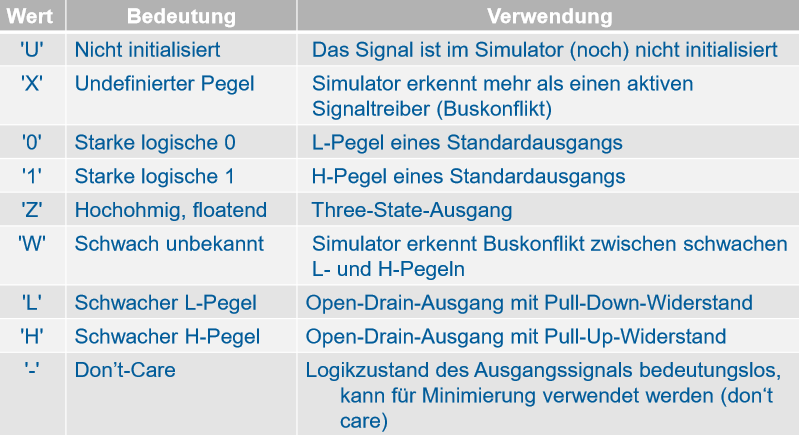
\includegraphics[width=\columnwidth]{Images/ieee_typen}
\end{center}
\textbf{std\_ulogic} akzeptiert nur einen Treiber pro Signal. Compiler erkennt Signalkonflikt und bricht mit Fehlermeldung ab.\\~\\
\textbf{std\_logic} akzeptiert mehrere Treiber pro Signal. Deshalb wird dieser Datentype für bidirektionale Busse eingesetzt. Entscheid, welcher Treiber sich durchsetzt, fällt der Simulator.
\begin{center}
	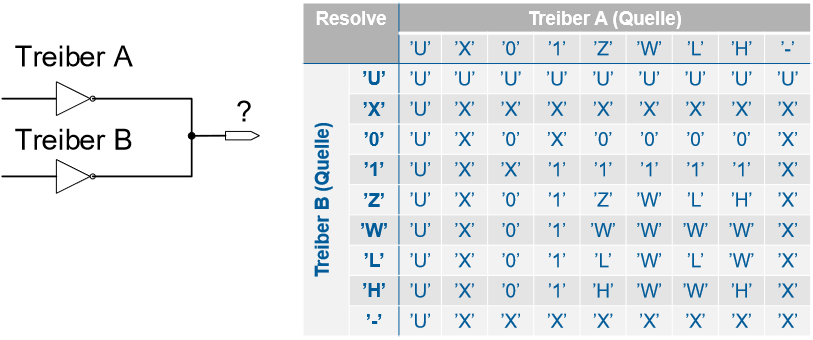
\includegraphics[width=\columnwidth]{Images/ieee_typen1}
\end{center}

\noindent\textbf{Type Cast}
\begin{center}
	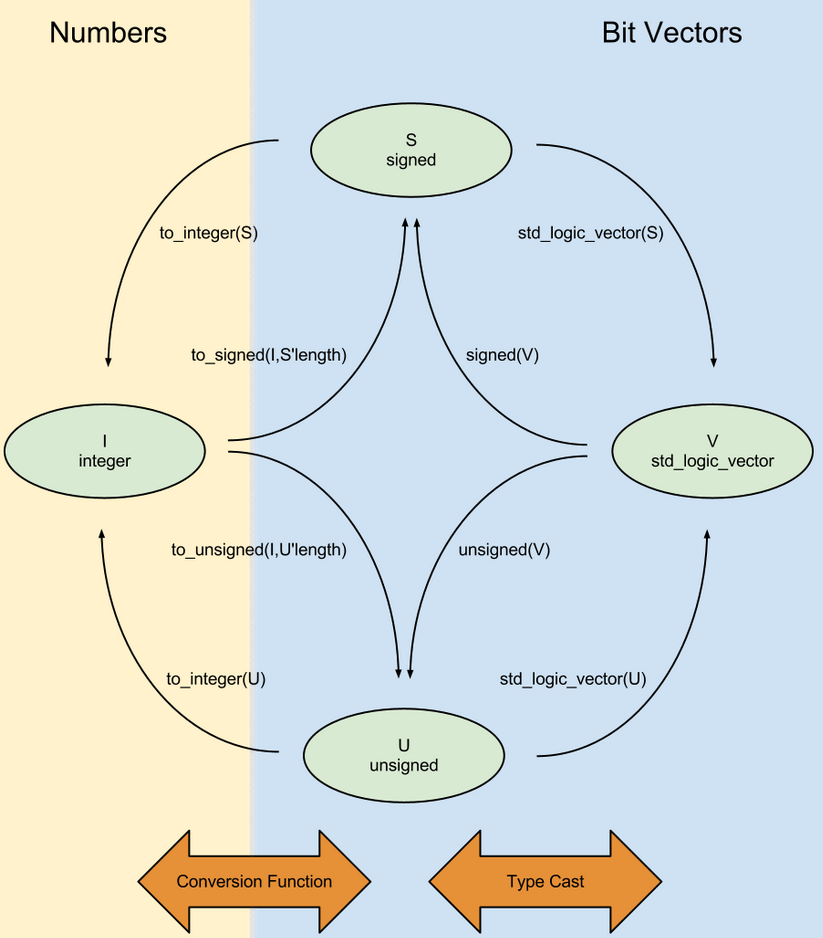
\includegraphics[width=0.8\columnwidth]{Images/type_cast}
\end{center}

\noindent\textbf{Operatoren}
\begin{center}
	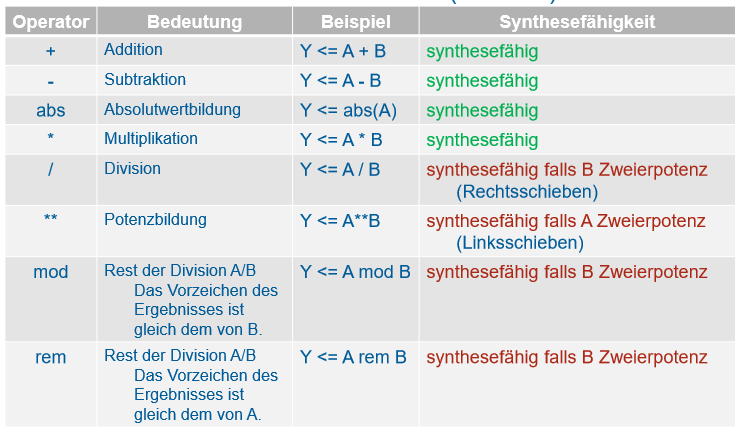
\includegraphics[width=\columnwidth]{Images/type_operator}
\end{center}
